%	This is written by Zhiyang Ong for the report proposal for ECEN 676 Advanced Computer Architecture, Fall 2014, at Texas A&M University.

%	The MIT License (MIT)

%	Copyright (c) <2014> <Zhiyang Ong>

%	Permission is hereby granted, free of charge, to any person obtaining a copy of this software and associated documentation files (the "Software"), to deal in the Software without restriction, including without limitation the rights to use, copy, modify, merge, publish, distribute, sublicense, and/or sell copies of the Software, and to permit persons to whom the Software is furnished to do so, subject to the following conditions:

%	The above copyright notice and this permission notice shall be included in all copies or substantial portions of the Software.

%	THE SOFTWARE IS PROVIDED "AS IS", WITHOUT WARRANTY OF ANY KIND, EXPRESS OR IMPLIED, INCLUDING BUT NOT LIMITED TO THE WARRANTIES OF MERCHANTABILITY, FITNESS FOR A PARTICULAR PURPOSE AND NONINFRINGEMENT. IN NO EVENT SHALL THE AUTHORS OR COPYRIGHT HOLDERS BE LIABLE FOR ANY CLAIM, DAMAGES OR OTHER LIABILITY, WHETHER IN AN ACTION OF CONTRACT, TORT OR OTHERWISE, ARISING FROM, OUT OF OR IN CONNECTION WITH THE SOFTWARE OR THE USE OR OTHER DEALINGS IN THE SOFTWARE.

%	Email address: echo "cukj -wb- 23wU4X5M589 TROJANS cqkH wiuz2y 0f Mw Stanford" | awk '{ sub("23wU4X5M589","F.d_c_b. ") sub("Stanford","d0mA1n"); print $5, $2, $8; for (i=1; i<=1; i++) print "6\b"; print $9, $7, $6 }' | sed y/kqcbuHwM62z/gnotrzadqmC/ | tr 'q' ' ' | tr -d [:cntrl:] | tr -d 'ir' | tr y "\n"

%%%%%%%%%%%%%%%%%%%%%%%%%%%%%%%%%%%%%%%%%%%%%%



%%%%%%%%%%%%%%%%%%%%%%%%%%%%%%%%%%%%%%%%%%%%%%
%	Preamble.
\documentclass[letter,12pt]{article}
%%%%%%%%%%%%%%%%%%%%%%%%%%%%%%%%%%%%%%%%%%%%%
%
%	Importing LaTeX source files, without quoting the ".tex" extension.
%
%%%%%%%%%%%%%%%%%%%%%%%%%%%%%%%%%%%%%%%%%%%%%

%%%%%%%%%%%%%%%%%%%%%%%%%%%%%%%%%%%%%%%%%%%%%
%	File containing the LaTeX preamble.
% This is written by Zhiyang Ong as the preamble for all his LaTeX documents.
%
% It includes a list of LaTeX packages that he commonly uses to typeset LaTeX documents.

%	The MIT License (MIT)

%	Copyright (c) <2014> <Zhiyang Ong>

%	Permission is hereby granted, free of charge, to any person obtaining a copy of this software and associated documentation files (the "Software"), to deal in the Software without restriction, including without limitation the rights to use, copy, modify, merge, publish, distribute, sublicense, and/or sell copies of the Software, and to permit persons to whom the Software is furnished to do so, subject to the following conditions:

%	The above copyright notice and this permission notice shall be included in all copies or substantial portions of the Software.

%	THE SOFTWARE IS PROVIDED "AS IS", WITHOUT WARRANTY OF ANY KIND, EXPRESS OR IMPLIED, INCLUDING BUT NOT LIMITED TO THE WARRANTIES OF MERCHANTABILITY, FITNESS FOR A PARTICULAR PURPOSE AND NONINFRINGEMENT. IN NO EVENT SHALL THE AUTHORS OR COPYRIGHT HOLDERS BE LIABLE FOR ANY CLAIM, DAMAGES OR OTHER LIABILITY, WHETHER IN AN ACTION OF CONTRACT, TORT OR OTHERWISE, ARISING FROM, OUT OF OR IN CONNECTION WITH THE SOFTWARE OR THE USE OR OTHER DEALINGS IN THE SOFTWARE.

%	Email address: echo "cukj -wb- 23wU4X5M589 TROJANS cqkH wiuz2y 0f Mw Stanford" | awk '{ sub("23wU4X5M589","F.d_c_b. ") sub("Stanford","d0mA1n"); print $5, $2, $8; for (i=1; i<=1; i++) print "6\b"; print $9, $7, $6 }' | sed y/kqcbuHwM62z/gnotrzadqmC/ | tr 'q' ' ' | tr -d [:cntrl:] | tr -d 'ir' | tr y "\n"

%%%%%%%%%%%%%%%%%%%%%%%%%%%%%%%%%%%%%%%%%%%%%%%%%%

% Importing some standard LaTeX packages.

% To enable standard LaTeX processing for graphics. It enables PDF, JPEG, PNG, and TIFF graphics files to be included in the LaTeX document.
\usepackage{graphicx}
% For better typesetting of mathematical expressions, from the American Mathematical Society (AMS).
\usepackage{amsmath}
% For better typesetting of mathematical expressions, from the American Mathematical Society (AMS). This package includes mathematical symbols for the ``amsmath'' package.
\usepackage{amssymb}
% For better typesetting of mathematical proofs (for theorems and colloraries), from the American Mathematical Society (AMS).
\usepackage{amsthm}
%	Create definitions for new theorems, axioms, colloraries.
	\newtheorem{theorem}{Theorem}[section]
	\newtheorem{axiom}{Axiom}[section]
	\newtheorem{corollary}{Corollary}[section]
	\newtheorem{lemma}{Lemma}[section]
	\newtheorem{Rule}{Rule}[section]
	\newtheorem{law}{Law}[section]
	\newtheorem{principle}{Principle}[section]
% To change the style of newly defined theorems.
%		\usepackage{theorem}


% For better typesetting of tables (and arrays).
\usepackage{array}
% For creating tables without vertical separators.
%		\usepackage{booktabs}
% To control line spacing in LaTeX documents.
\usepackage{setspace}
% To modify the spacing between words and letters.
%		\usepackage{microtype}
% To change the dimensions of the page(s).
%\usepackage[margin=1.5cm,vmargin={0pt,1cm},nohead]{geometry}
\usepackage[margin=1.5cm,vmargin={1.5cm,2cm}]{geometry}
% Use the packages needed to typeset algorithms. I can also use the combined ``algorithms'' bundle.
\usepackage{algorithm}
\usepackage{algorithmic}
% The listings package is a source code printer for LaTeX. You can typeset stand alone files as well as listings with an environment similar to verbatim as well as you can print code snippets using a command similar to \verb. Many parameters control the output and if your preferred programming language isn�t already supported, you can make your own definition.
\usepackage{listings}
% Use the ``clrscode3e'' LaTeX package to typeset algorithms like CLRS
%	\usepackage{/data/others/notes/clrscode3e}
\usepackage{/data/others/grappanotes/clrscode3e}
% Use the ``algpseudocode'' LaTeX package to typeset algorithms -- Alternate solution, not preferred
%\usepackage{algpseudocode}
% Alternative packages for typesetting algorithms.
%\usepackage{algorithm2e}
%\usepackage{algorithmicx}
%\usepackage{program}
%	To check for syntax errors in my LaTeX document.
\RequirePackage[l2tabu, orthodox]{nag}

% Concatenate adjacent references together when typeset.
% That is, cite{ref1,ref2,ref3,ref4} can appear as [12-15], instead of [12] [13] [14] [15]
\usepackage{cite}
% For automatic insertion of cross-referencing words, such as fig. for figures and eq. for equations.
%		\usepackage{cleveref}

% LaTeX support for Metafont and MetaPost logos.
\usepackage{mflogo}













% How to typeset single and double quotes for feet and inches?
% For feet, use [FEET]\textasciiacute
% For inches, use [INCHES]\textacutedbl
% For feet and inches, use [FEET]\textasciiacute\ [INCHES]\textacutedbl; force a character space between the single quote for feet and the height of the object in inches
% Don't use \textceltpal as a single quote to represent height in feet, or double \textceltpal (two concatenated \textceltpal) as a double quote to represent height in inches
% For double quotes, don't use two single quotes provided by the default settings of LaTeX. The resultant double quotes will be curly.

% The tipa package is for Phonetic Symbols -- I wanna use the \textceltpal symbol to represent a single quote, instead of using the generic ``curly'' single quote from \LaTeX (Table 10, pp.10)
\usepackage{tipa}
% The textcomp package is for Diacritics -- I wanna use the \textacutedbl symbol to represent a double quote (Table 28, pp.17), instead of using the generic ``curly'' double quotes from \LaTeX; however, when this symbol is used, I must force a character space to exist after the symbol by using the backslash followed by a character space. This package also provides the symbol for Copyleft, \textcopyleft, which is not available in LaTeX by default, and provides better looking symbols for: copyright, registered, and trademark (Table 33, pp.18). Also, it provides symbols for: \textcelsius, \textmho, \textmu, \textohm (Table 201, pp.67). It also provides symbols for Genealogical Symbols (Table 253, pp78), such as \textborn, \textdivorced, \textmarried, \textdied, and \textleaf (symbol of a leaf)... Its symbol for the Euro, EU currency, is \texteuro
\usepackage{textcomp}
% Look at \url{http://www.ctan.org/tex-archive/info/symbols/comprehensive/symbols-a4.pdf} for a list of symbols that can be used in LaTeX and its packages. Table 280, pp.88, deals with Symbol Name Clashes; hence, if the same command name refers to multiple symbols, the symbol-conflict resolution abides by this.
% In particular, check out the gensymb package (Table 197, page 67) for symbols defined to work in both math and text modes, such as \celsius, \micro, \degree, and \ohm.
% Also, check out the wasysym package (Table 198, page 67) for electrical symbols, such as that of alternating current (AC); it also provides symbols for \female, and \male (Table 212, pp.70); it also has symbols for ``Xs and Check Marks,'' which are checked boxes, \CheckedBox, squares, \Square, and crossed boxes (boxes filled with a cross), \XBox (Table 232, pp.73); it also has symbols for a clock, \clock, a Simley, \smiley, diameter, \diameter, lightning, \lightning, sun, \sun, and a tick or check mark \checked (symbol to indicate that something is correct), and a bell, \bell (Table 254, pp.78); it also has symbols for left and right turns (Table 256, pp.78), \leftturn and \rightturn; this package (Table 256, pp.78) and the arev package (Table 257, pp.78) can be used to typeset music symbols, along with Table 182, pp.62; it also has symbols for Navigation (Table 261, pp.79), such as \Forward, \RewindToStart, and \ForwardToIndex; it also has symbols for laundry (Table 262, pp.80); it also has the symbol for a heart, \Heart (Table 263, pp.80).
% In addition, check out the ifsym package (Table 199, page 67) for pulse diagram symbols; it also has symbols for weather (Table 266, pp.80), alpine and mountain climbing, such as \Summit, \Mountain, \IceMountain, \VarMountain, \Flag, \FilledHut, \Hut, \Village, and \Tent (Table 267, pp.81); it also has different symbols for clocks, such as \Interval, \StopWatchEnd, \VarClock, \showclock (to indicate the time) (Table 268, pp.81); it also has symbols for fire, letter, telephone, dice, \PaperPortrait, and \PaperLandscape. Also, has symbol for the cross to indicate that something is incorrect
\usepackage{ifsym}
% Besides, check out the keystroke package (Table 208, page 69) for symbols of Computer Keys, such as Alt, Ctrl, Del, Page down, Esc, Enter, Shift, Space Bar, and Up Arrow.
% From the dingbat package (Table 225, page 72), it has symbols for Fists, such as \rightthumbsdown and \rightthumbsup.
%\usepackage{dingbat}
% From the pifont package (Table 234, page 73), it has symbols for Circled Numbers, such as any digit that is circled, where the space in the circle can be shaded black.
% From the dictsym package (Table 277, page 84), it has symbols for dictionaries, and indicates which type of dictionary will define this term - say a medical, technical, mathematical, or judical dictionary
% The simpsons package can be used to indicate characters from {\it The Simpsons} (Table 278, pp.85)
% The symbol for quadruple integrals \iiiint is available as an AMS Variable-sized Math Operator, or I can use this symbol from the packages txfonts, pxfonts, esint, or MnSymbol 










% The marvosym package (Table 210, page 69) is for Communication Symbols, such as \Email, \fax, \FAX (Preferred), \Letter, \Mobilefone, and \Telefon; it also has the symbol for the Cross to represent Christianity, \Cross (Table 263, pp.80); it also has symbols for checked boxes, \Checkedbox, crossed boxes (boxes marked with a cross), \Crossedbox, bicycles, \Bicycle, clocks, \Clocklogo, the industry, \Industry, taking notes manually with pen/pencil and paper, \Writinghand, coffee, \Coffeecup, providing information or important note, \Info (Table 249, pp.76)... In addition, it has the symbols for the Euro (EU currency), \EUR (OK), \EURdig (OK), \EURtm, \EURcr
\usepackage{marvosym}
% From the bbding package (Table 226, page 72), it has symbols for Fists, such as \HandPencilLeft; it also has symbols for the Cross to represent Christianity, such as \Cross and \CrossOpenShadow (Table 228, pp.72); Use of the symbol \Cross has bugs; bugs exist in the package, as it fails to correctly overwrite the \Cross symbol; also has the peace symbol, \Peace. 
%\usepackage{bbding}
% The skak contains a cross, incorrect symbol that I can use to indicate that something is wrong, e.g. \markera or \weakpt
\usepackage{skak}
% Package to enable the use of a strikeout/strikethrough font with LaTeX. To use the strikeout/strikethrough font, use the ``sout'' LaTeX command, or tag,  to ``strike through'' text. E.g., \sout{Bill Clinton} G.W. Bush is the pres.
\usepackage{ulem}
% The eurosym package has the symbols for the Euro (EU currency), \geneuro, \geneuronarrow, \geneurowide, \officialeuro (GOOD)
\usepackage{eurosym}











% Create fancy headers and footers for this document
\usepackage{fancyhdr}
\setlength{\headheight}{15.2pt}
\pagestyle{fancy}
% Headers for the document
\lhead{}
%\lhead{Zhiyang Ong}
%\rhead{\today}
% Footers for the document
\lfoot{Zhiyang Ong}
\cfoot{}
\rfoot{\thepage}

% The following does not work, since it does not differentiate between odd and even pages. Hence, the last odd/even command will overwrite the previous even/odd command
%\fancyhf{}
%\fancyhead[LE]{Author's DFM}
%\fancyhead[LO]{\today EDA}
%\fancyfoot[LE]{\thepage USC}
%\fancyfoot[RO]{\thepage Adel}


% Allow for multi-line comments
\usepackage{verbatim}




% Commands for using the package for hyperlinks. Includes the package ``url''.
\usepackage[pdftex,
	pdftitle={Graphics and Color with LaTeX},
	pdfauthor={Patrick W Daly},
	pdfsubject={Importing images and use of color in LaTeX},
	pdfkeywords={LaTeX, graphics, color},
	pdfpagemode=UseOutlines,bookmarks, bookmarksopen,
	pdfstartview=FitH, colorlinks, linkcolor=blue, citecolor=blue, urlcolor=red,
]{hyperref}
\hypersetup{colorlinks, linkcolor=blue}







% Create a glossary for symbols and terms in this document
% The following attempt failed
%\makeglossaries

% The following attempt failed
%%%%%%%%%%%%%%%%%%%%%%%%%%%%%\makeglossary
%\usepackage{supertabular}
%\newcommand{\glossaryname}{Symbols Index}
%\newenvironment{theglossary}
%    {\section*{Symbols Index}
%      \begin{supertabular}{ll}}
%    {\end{supertabular}
%}
%\newcommand{\printglossary}{\InputIfFileExists{zhiyang_ong.glo}{}{\section*{Symbols Index - File not found}}}

% Another failed attempt at creating a glossary
%\input{gatech-thesis-gloss.sty}
%\usepackage{gatech-thesis-gloss}
%\glossfiles{zhiyang_ong.glo}

% Create the glossary
\usepackage{nomencl}
\makenomenclature


% Enable captions to be modified.
%\usepackage{caption}
% Addition support for colored text.
%\usepackage{color}
% Enable the insertion of PDF/PS files/documents.
		\usepackage{pdfpages}
% To rotate objects, including tables.
		\usepackage{rotating}
% To define multiple floats (figures and tables), with individual captions and labels, within one environment.
		\usepackage{subfig}
% For a modular LaTeX document with multiple files (including the ``root file''), it allows the a non-empty subset of the ``child files'' to be typeset without having to typeset the ``root file'' (and/or the other ``child files'').
		\usepackage{subfiles}
% To annotate the LaTeX document with to-do notes.
		\usepackage[colorinlistoftodos]{todonotes}
% To insert images surrounded by text.
		\usepackage{wrapfig}
% To create trees, graphs, (commutative) diagrams, and similar things. Reference: Wikibooks contributors, ``\LaTeX/Xy-pic,'' in {\it \LaTeX}, Wikibooks: Open books for an open world, Wikimedia Foundation, San Francisco, CA, June 5, 2005. Available online at: \url{http://en.wikibooks.org/wiki/LaTeX/Xy-pic}; last accessed on December 25, 2013.		=> This package seems to have bugs in it. If I use this package, my document will not typeset properly. I have tried to use it successfully in other documents. It does not seem to be compatible with 
%\usepackage{xypic}
% Package for SI units.
\usepackage{siunitx}








%%%%%%%%%%%%%%%%%%%%%%%%%%%%%%%%%%%%%%%%%%%%%%%%%%
% Other helpful hints:

% To use the italic and bold font concurrently, try this: {\itshape Review the {\bfseries updated} training log}

% To use the symbol for summation, which is the capital-sigma notation, with proper super- and sub- fixes, try: $\displaystyle\sum_{i = -1}^{m} \frac{log_2 n_i}{T_i}$

% Make sure that I include the following so that I can cite references properly: \usepackage{cite}. This allows references to be included as [1-10], rather than [1], [2], [3], [4], [5], [6], [7], [8], [9], [10]

% Colors that appear well in PDF format for LaTeX text include: red, blue, and magenta

% Use \scriptsize, instead of \textsc, \sc, or \schape to use small caps. Currently, I cannot use \textsc, \sc, or \schape to write in small caps on my MacBook Pro laptop.

% The Typewriter font cannot be used concurrently with the bold font. That is, the following cannot be used: {\tt \bf text}, AND \texttt{\textbf{text}}

% Use \LaTeX for LaTeX; B{\scriptsize IB}\TeX to indicate the symbol for BibTeX; \texttrademark for trademarks; \MF for Metafont; and \MP for MetaPost




%%%%%%%%%%%%%%%%%%%%%%%%%%%%%%%%%%%%%%%%%%
%																%
%	Default colors that I can use with \LaTeX:								%
%	1) red														%
%	2) green														%
%	3) blue														%
%	4) yellow														%
%	5) cyan														%
%	6) magenta													%
%	7) black														%
%	8) white														%
%																%
%%%%%%%%%%%%%%%%%%%%%%%%%%%%%%%%%%%%%%%%%%


% Partial list of ``the 68 predefined internal colors of the {\tt dvips} PostScript driver'' \cite{Kopka04} that I can use for changing the color of text ... Use bold font for the text
%YellowOrange
%RoyalBlue
%DarkOrchid
%ForestGreen
%OliveGreen
%Mulberry
%ProcessBlue
%RubineRed
%VioletRed
%WildStrawberry
% E.g., try: \textcolor{VioletRed}{\bf hello world}

% As for changing the background color of text, choose a light colored background to make the text stand out in black colored bold font; see \url{oregonstate.edu/~peterseb/tex/samples/docs/color-package-demo.pdf} for a list of colors
% E.g., try: \colorbox{Apricot}{\bf hello world}





% definition of new \LaTeX command for the citation: \cite{Cimatti08} and \cite{Barrett09}
% This allows mathematical/logic symbols to be typeset with the font ``Zapf Chancery'' in ``\LaTeX\ math mode''. To typeset symbols in such font, try: \mathpzc{ABCdef123}
\DeclareMathAlphabet{\mathpzc}{OT1}{pzc}{m}{it}

%%%%%%%%%%%%%%%%%%%%%%%%%%%%%%%%%%%%%%%%%%%%%
% Start of document
\begin{document}
\title{Proposal for Report on Processor Architectures}
\author{}
\date{}
%\author{Zhiyang Ong}
%\date{\today}
%\author{Nithin Poduval, Yangzheng Bai, Zhiyang Ong,\\ and Alberto Javier Naranjo Carmona}
%\author{Yangzheng Bai, Zhiyang Ong,\\ and Alberto Javier Naranjo Carmona}
\maketitle



%\begin{abstract} 
%This is a set of guidelines for conduct for the Aggietects team. It also includes guidelines for creating a shared {\sc Bib}\TeX\ database.
%\end{abstract}

\vspace{-0.5in}
\ \\
To: Prof. Richard McGuire \\
From: Zhiyang Ong \\
Date: October 9, 2014 \\

%	Table of Contents
\tableofcontents
%\newpage
%\addcontentsline{toc}{subsection}{Preface}


%%%%%%%%%%%%%%%%%%%%%%%%%%%%%%%%%%%%%%%%%%%
%	Begin left-alignment
\begin{flushleft}


%%%%%%%%%%%%%%%%%%%%%%%%%%%%%%%%%%%%%%%%%%%
\section{Introduction to Processor Architecture}
\label{sec:ProcessorArchitecture}

In this section, I provide the motivation to write a report on processor architecture, and introduction to processor architecture. \\
\ \\
Current and emerging trends in ``Big Data'' \cite{BilbaoOsorio2014,Wedewer2013}, Internet of Things \cite{Witchalls2013}, and cyber-physical systems \cite{PCAST2013} drives a need for energy-efficient computing. From mobile devices to high-performance super computing, the cost of power and cooling these computers have become so dominant that they have become a barrier to improving the performance of computers \cite{Hennessy2012,Fuller2011}. Without better computers, it can be harder for companies to sell computers to consumers and enterprises. Furthermore, computer architecture is a difficult subject to teach, especially at the undergraduate level \cite{Yurcik2002}. Due to the demand for high-performance, energy-efficient processors \cite{Duranton2013}, we need to train more highly-skilled computer engineering students to pursue a career in the field of computer architecture. In addition, before students and professionals can tackle grand challenges in computer architecture \cite{Track2014}, they need to master the basics of modern processor design. \\
%Current and emerging trends in ``Big Data'' \cite{BilbaoOsorio2014,Wedewer2013,Agrawal2012,Manyika2011a}, Internet of Things \cite{Witchalls2013}, and cyber-physical systems \cite{PCAST2013} drives a need for energy-efficient computing. From mobile devices to high-performance super computing, the cost of power and cooling these computers have become so dominant that they have become a barrier to improving the performance of computers \cite{Hennessy2012,Fuller2011}. Without better computers, it can be harder for companies to sell computers to consumers and enterprises. Furthermore, computer architecture is a difficult subject to teach, especially at the undergraduate level \cite{Yurcik2002}. Due to the demand for high-performance, energy-efficient processors \cite{Duranton2013,Manyika2013,Wedewer2013}, we need to train more highly-skilled computer engineering students to pursue a career in the field of computer architecture. In addition, before students and professionals can tackle grand challenges in computer architecture \cite{Track2014}, they need to master the basics of modern processor design. \\
\ \\
Processor architecture refers to the structure and organization of the computer chip (or processor), including the set of instructions that it can comprehend \cite{Hennessy2012}. The study of this is critical to designing faster computers, reducing energy consumption of computers, and improving the reliability of computers. It also defines the hardware and software interface \cite{Patterson2014}, so that engineers designing computer hardware and software developers can collaborate or work independently to create compelling products for customers and end users.





%%%%%%%%%%%%%%%%%%%%%%%%%%%%%%%%%%%%%%%%%%%
\section{Description of the Report}
\label{sec:DescriptionoftheReport}

In this section, a structure for the report is described. In Subsection \ref{ssec:AudienceandPurpose}, we specify the audience and purpose of the report proposal and the report. Following that in Subsection \ref{ssec:TentativeOutline}, we provide a tentative outline of the report. Lastly, in Subsection \ref{ssec:PreliminaryBibliography}, we provide a preliminary bibliography for the report.

%%%%%%%%%%%%%%%%%%%%%%%%%%%%%%%%%%%%%%%%%%%
\subsection{Audience and Purpose}
\label{ssec:AudienceandPurpose}

The sole audience of the report proposal and a primary audience for the report is Prof. Richard McGuire. Secondary audience for the report would include my peers and myself, who can use the report to help them review the basics of processor architecture for their classes on computer architecture. We (my peers and myself) can also use the report to help us prepare for the Ph.D. qualifying examination, or equivalent, and for job interviews. Tertiary audience would include undergraduates who want to learn about processor architecture design, so that they can engage in undergraduate research projects and consider going to graduate school or pursue an engineering career in computer architecture. Since processor architecture is poorly taught in many universities, this is important in the context of broadening participation of not-so-privileged students in processor architecture.

%%%%%%%%%%%%%%%%%%%%%%%%%%%%%%%%%%%%%%%%%%%
\subsection{Tentative Outline}
\label{ssec:TentativeOutline}

A tentative outline for the structure of the report is given as follows, with annotations to describe the importance and relevance of each section.

\begin{enumerate} \itemsep -4pt
\item Introduction. {\it This section introduces processor architecture, and basic concepts in processor architecture (or  microarchitecture) and some background information.}
\item Single-cycle processor. {\it This section describes how to design the most basic type of processor architecture}
\item Multi-cycle processor. {\it This section describes a faster microarchitecture, which allocates multiple clock cycles for each instruction.}
\item Pipelined processor. {\it This section describes an even faster microarchitecture based on the notion of pipelining.}
\item Out-of-order pipelined processor. {\it This section describes a microarchitecture that rearranges instructions of a computer program to improve performance.}
\item Out-of-order superscalar processor. {\it This section addresses contemporary microarchitectures by issuing multiple instructions per clock cycle to improve performance.}
\item Conclusion. {\it This section concludes the report by summarizing the basic concepts in processor architecture and providing some directions for more advanced work in processor architecture.}
\end{enumerate}

%%%%%%%%%%%%%%%%%%%%%%%%%%%%%%%%%%%%%%%%%%%
\subsection{Preliminary Bibliography}
\label{ssec:PreliminaryBibliography}

My preliminary bibliography is listed below with annotations. For each publication, I would indicate the publication followed by a brief explanation of why I am using that publication. \vspace{-0.3cm}
\begin{enumerate} \itemsep -4pt
\item John L. Hennessy and David A. Patterson, ``Computer Architecture: A Quantitative Approach,'' Fifth edition, Morgan Kaufmann, 2012. \\
\ \\
This is the seminal textbook on modern computer architecture, including processor architecture. It addresses the most important concept in processor architecture, and other related aspects of computer architecture. It has worked examples and exercises to help people learn contemporary concepts in computer architecture. It covers current and emerging trends in processor architecture, and analyzes some modern processors to help readers see how advance concepts of processor architecture are used in commercial products.
%http://booksite.mkp.com/9780123838728/index.php
%\cite{Hennessy2012}
\item David A. Patterson and John L. Hennessy, ``Computer Organization and Design: The Hardware/Software Interface,'' Fifth edition, Morgan Kaufmann, Waltham, MA, 2014. \\
\ \\
This book is a seminal textbook to the fundamentals of computer architecture, including processor architecture. It provides adequate details to enable readers to design their own processors using technologies developed in the 1980s. It has worked examples and exercises for readers to test their knowledge of processor architecture, and related topics.
%Patterson2014
\item David Money Harris and Sarah L. Harris, ``Digital Design and Computer Architecture,'' Morgan Kaufmann,Waltham, MA, 2007. \\
\ \\
This book introduced the basic concepts of processor architecture, circa the 1980s, such as pipelined reduced instruction set computing (RISC) processors. It includes examples and exercises to help us learn the material. Furthermore, it includes material on logic design to help us implement the microarchitecture of simple processors, circa the 1980s.
%Harris2007
%\item Silvia Melitta Mueller and Wolfgang J. Paul, ``Computer Architecture: Complexity and Correctness,'' Springer-Verlag Berlin Heidelberg, Heidelberg, Germany, 2000. \\
%\ \\
%This books covers the basic design flow of processor architectures, and the basic concepts of processor architecture. It also includes exercises to help readers test their concepts of processor architecture.
%Mueller2000
\end{enumerate}



Some ancillary publications that may help me explain various concepts of modern processor architecture design to engineering and computer science students and junior professionals are listed as follows. \vspace{-0.3cm}
\begin{enumerate} \itemsep -4pt
%\item Mostafa Abd-El-Barr and Hesham El-Rewini, ``Fundamentals of Computer Organization and Architecture,'' Wiley Series in Parallel and Distributed Computing, John Wiley \& Sons, Hoboken, NJ, 2005. \\
%\ \\
%This book covers the basics of computer organization without too much technical details and rigor. However, it is highly superficial in describing the microarchitecture of processors. Therefore, it is difficult to design and implement the microarchitecture of a processor, without referring to better books on processor architecture.
%\cite{AbdElBarr2005}
\item Rajeev Balasubramonian and Norman P. Jouppi and Naveen Muralimanohar, ``Multi-Core Cache Hierarchies,'' Synthesis Lectures on Computer Architecture series, Morgan \& Claypool Publishers, San Rafael, CA, November, 2011. \\
\ \\
This book covers advanced material on hierarchical cache design for multi-core processors. However, it does not provide the basics for simple cache design for single-core/uni- processors. It also does not cover other topics in processor architecture design. Given its brevity on advanced topics, lack of examples, and lack of exercises (or problem sets) to help us learn concepts, I do consider it as a primary resource for architecture resource. That said, it is a helpful secondary resource for advanced topics in multi-core processors.
%\cite{Balasubramonian2011}
%\item Hesham El-Rewini and Mostafa Abd-El-Barr, ``Advanced Computer Architecture and Parallel Processing,'' Wiley Series in Parallel and Distributed Computing, John Wiley \& Sons, Hoboken, NJ, 2005. \\
%\ \\
%This book provides some qualitative basic information about parallel computing, and does not include detailed information to implement chip multiprocessors. The book has some problems at the end of each chapter to test our concepts, but it does not include worked examples.
%\cite{ElRewini2005}
%\item Antonio Gonz{\'{a}}lez, Fernando Latorre, and Grigorios Magklis, ``Processor Microarchitecture: An Implementation Perspective,'' Synthesis Lectures on Computer Architecture series, Morgan \&\ Claypool Publishers, San Rafael, CA, December, 2010. \\
%\ \\
%It covers the basics of processor architecture, such as: Flynn's taxonomy for classifying processor architectures, pipelined processor architectures, and component design for each pipelined stage of a simple microarchitecture design. However, this monograph is lacking in implementation details for the design of a processor architecture. It also does not have worked examples nor problems to help us learn.
%Gonzalez2010
\item Stephen W. Keckler and Kunle Olukotun and H. Peter Hofstee, ``Multicore Processors and Systems,'' Integrated Circuits and Systems series, Springer Science+Business Media, LCC, New York, NY, 2009. DOI: http://dx.doi.org/10.1007/978-1-4419-0263-4. \\
\ \\
This book covers contemporary trends in multicore processor architectures. However, it does not cover the design flow of processor architecture, which is important to help people get an overview of how to design multicore processors. In addition, it also does not have worked examples nor exercises to help students learn about multicore processor design.
%Keckler2009
\item Vojin G. Oklobdzija and Ram K. Krishnamurthy, ``High-Performance Energy-Efficient Microprocessor Design,'' Integrated Circuits and Systems series, Springer, Dordrecht, The Netherlands, 2006. \\
\ \\
This covers some contemporary topics in processor design, but does not contain adequate information to help readers acquire the basics and the design flow of processors. Readers of this book are expected to have a significant background in processor design.
%Oklobdzija2006
%\item Kunle Olukotun, Lance Hammond, and James Laudon, ``Chip Multiprocessor Architecture: Techniques to Improve Throughput and Latency,'' Synthesis Lectures on Computer Architecture series, Morgan \&\ Claypool Publishers, San Rafael, CA, 2007. \\
%\ \\
%This book covers some advance topics in processor architecture, but does not provide worked examples nor exercises to help readers learn material about the topics.
%Olukotun2007
%\item Amos R. Omondi, ``The Microarchitecture of Pipelined and Superscalar Computers,'' Kluwer Academic Publishers, Dordrecht, The Netherlands, 1999. \\
%\ \\
%This book covers some aspects of advanced processor architectures, but does not thoroughly provide details about those aspects nor provide worked examples and exercises to help readers learn. It also does not give users a good overview of the processor design process.
%Omondi1999
%\item Daniel Page, ``A Practical Introduction to Computer Architecture,'' Texts in Computer Science series, Springer-Verlag London, London, U.K., 2009. \\
%\ \\
%This book has a good overview of processor architecture, and lacks adequate depth to use this as a sole resource to design a processor.
%Page2009
%\item Sajjan G. Shiva, ``Advanced Computer Architectures,'' CRC Press, Boca Raton, FL, 2006. \\
%\ \\
%This book covers some advanced concepts of computer architecture, but lacks a good overview of the process of designing processors. 
%Shiva2006
%\item Sajjan G. Shiva, ``Computer Organization, Design, and Architecture,'' Fourth edition, CRC Press, Boca Raton, FL
%2007 \\
%\ \\
%This provides a good overview of logic design and computer architecture, and includes worked examples and problems to help us learn the basic concepts.
%Shiva2007
%\item Jurij {\v{S}}ilc, Borut Robi{\v{c}}, and Theo Ungerer, ``Processor Architecture: From Dataflow to Superscalar and Beyond,'' Springer-Verlag Berlin Heidelberg, Heidelberg, Germany, 1999. \\
%\ \\
%This book provides a good overview of processor architecture, categories thereof, and current processor architecture trends. However, it does not include worked examples or exercises to help us acquire new techniques and solutions.
%Silc1999
%\item Daniel J. Sorin, ``Fault Tolerant Computer Architecture,'' Synthesis Lectures on Computer Architecture series, Morgan \&\ Claypool Publishers, San Rafael, CA, 2009. \\
%\ \\
%The book focuses on error detection and correction, error diagnosis, and self-repair. It does not have a good overview of processor architecture, but covers adequate techniques for fault-tolerant computing. Hence, apart from the advance topic of fault-tolerant computing, it does not cover enough details of processor architecture to help readers design their own processors.
%Sorin2009
%\item Stallings, William, ``Computer Organization and Architecture: Designing for Performance,'' Eighth edition, Prentice Hall, Upper Saddle River, NJ, 2012. \\
%\ \\
%It provides a good overview of computer architecture and has exercises to test our knowledge, but lacks worked examples to help us apply our knowledge. It also lacks detailed information on designing processor architecture, using contemporary technologies and techniques.
%Stallings2012
%\item Andrew S.Tanenbaum, ``Structured Computer Organization,'' Sixth edition, Prentice-Hall, Upper Saddle River, NJ, 2013. \\
%\ \\
%This book does provide a good overview of processor architecture, along with other aspects of computer architecture and related topics (such as operating systems and computer networks). However, it lacks worked examples to complete the lists of exercises at the end of each chapter. 
%Tanenbaum2013
%\item Rob Williams, ``Computer Systems Architecture: A Networking Approach,'' Pearson Education, Upper Saddle River, NJ, 2006.
%This book is too generic, and covers computer systems and computer networks, and operating systems.
%Williams2006
%\item Wayne Wolf, ``High-Performance Embedded Computing: Architectures, Applications, and Methodologies,'' Morgan Kaufmann, San Francisco, CA, 2007. \\
%\ \\
%While it provides a good overview to high-performance embedded system design, it does not have enough information on processor design. In addition, while it has exercises for students to practice what they have learned, there is no worked examples for students to self-test.
%Wolf2007,
\item Tim Harris, James Larus, Ravi Rajwar, ``Transactional Memory,'' Synthesis Lectures on Computer Architecture series, Morgan \& Claypool Publishers, San Rafael, CA, Second edition, December 2010. \\
\ \\
This book provides an introduction into a special topic, transactional memory, and addresses it from a parallel programming approach. Hence, it addresses the lack of coverage of transactional memory in other references from a modern perspective.
%Harris2010a
%B. Falsafi and T. F. Wenisch. A Primer on Hardware Prefetching. Synthesis Lectures on Computer Architecture. Morgan & Claypool Publishers, San Rafael, CA, May 2014.
%Falsafi2014
%\item L. Eeckhout. Computer Architecture Performance Evaluation Methods. Synthesis Lectures on Computer Architecture. Morgan & Claypool Publishers, San Rafael, CA, December 2010.
%\ \\
%This book covers the basics of performance evaluation for computer architectures/systems, and the performance metrics that shall be used for such performance estimation. It also addresses multi-threaded and multi-program workload evaluation, and how to design workloads for performance benchmarking. In addition, it covers analytical techniques and models for performance analysis, and simulation techniques (such as statistical simulation, sampled simulation, parallel simulation, and hardware acceleration) for performance analysis.
%Eeckhout2010
%\item B. Jacob. The Memory System: You Can�t Avoid It, You Can�t Ignore It, You Can�t Fake It. Synthesis Lectures on Computer Architecture. Morgan & Claypool Publishers, San Rafael, CA, 2009.\\
%B. Jacob, S. Ng, and D. Wang. Memory Systems: Cache, DRAM, Disk. Elsevier Inc., Burlington, MA, 2008.\\
%\ \\
%These references provide additional information on designing the memory systems of computers, which significantly contribute to the performance of the computer system.
%Jacob2009
\end{enumerate}










%%%%%%%%%%%%%%%%%%%%%%%%%%%%%%%%%%%%%%%%%%%
\section{Project Plan}
\label{sec:ProjectPlan}

This section introduces how the project of writing my report shall be planned. In Subsection \ref{ssec:TasksandMethods}, I would discuss the tasks and subtasks that need to be completed to finish writing my report, and the methods that I would use to complete the tasks. This subsection would also include milestones that need to be completed. Subsequently, in Subsection \ref{ssec:Schedule}, I would discuss the schedule for the milestones of this report writing process. Lastly, in Subsection \ref{ssec:RiskManagement}, risk management is carried out to determine the risks involved in the report writing process.

%%%%%%%%%%%%%%%%%%%%%%%%%%%%%%%%%%%%%%%%%%%
\subsection{Tasks and Methods}
\label{ssec:TasksandMethods}

The tasks of writing the report would include some literature review of the books regarding computer architecture, as well as going over worked examples and solving exercises in the textbook to help me improve my knowledge of processor architecture design. It also includes designing a processor to test my concepts in processor architecture, and running processor simulators to examine how would changing the parameters of a processor affect its performance and power consumption. For the primary concepts involved in design processors, I would include a section to describe them in my report. \\
\ \\
The aforementioned tasks and proposed methods to accomplish these tasks are listed below. \vspace{-0.3cm}
\begin{enumerate} \itemsep -4pt
\item Literature review of some books about computer architecture
%\item Comprehend worked examples and solve exercises in textbooks to help me improve my knowledge of processor architecture design. I shall cover the following on the following topics: %\vspace{-0.3cm}
%	\begin{enumerate} %\itemsep -2pt
%	\item Single-cycle processor
%	\item Multi-cycle processor
%	\item Pipelined processor
%	\item Out-of-order pipelined processor
%	\item Out-of-order superscalar processor
%	\end{enumerate}
%\item Designing a processor to test my concepts in processor architecture
%\item Running processor simulators to examine how would changing the parameters of a processor affect its performance and power consumption
\item Single-cycle processor section
\item Multi-cycle processor section
\item Pipelined processor section
\item Out-of-order pipelined processor section
\item Out-of-order superscalar processor section
\item Report writing
\item Progress report
\item Review drafts of report
\end{enumerate}

Progress reports are due according to dates set in the course syllabus, but are subject to be rescheduled upon the recommendation of the course instructor, Prof. Richard McGuire. Drafts for my report, segmented by sections can be completed and reviewed by my peers. Completing drafts on schedule, as indicated in Figure \ref{fig:ganttchart}, would enable me to stay on track and mitigate the risk of having to complete the report in rush just before the deadline. Each section shall be completed with a write-up for that section, so that the report would be a concatenation of these sections. For the each section, I shall comprehend worked examples from the textbooks and solve exercises in them. For the single-cycle processor and pipelined processor, I would simulate them with processor simulators and design them as integrated circuits. These activities would help me explain the basics of processor architecture better.



%%%%%%%%%%%%%%%%%%%%%%%%%%%%%%%%%%%%%%%%%%%
\subsection{Schedule}
\label{ssec:Schedule}

In this section, I briefly describe the schedule for the report writing process. In Figure \ref{fig:ganttchart}, the Gantt chart shows the schedule for managing my report writing process. It indicates that the time frame in which I expect to complete the main tasks of the report. Since the concepts for single-cycle processors, multi-cycle processors, and pipelined processors are easier than out-of-order pipelined processors and out-of-order superscalar processors, I would cover these material in a week each. As for out-of-order pipelined processors and out-of-order superscalar processors, I need more time to elaborate the details involved in designing these modern processor architectures. Hence, I have set aside two weeks for each of these sections.

\begin{figure}[h]
\centering 
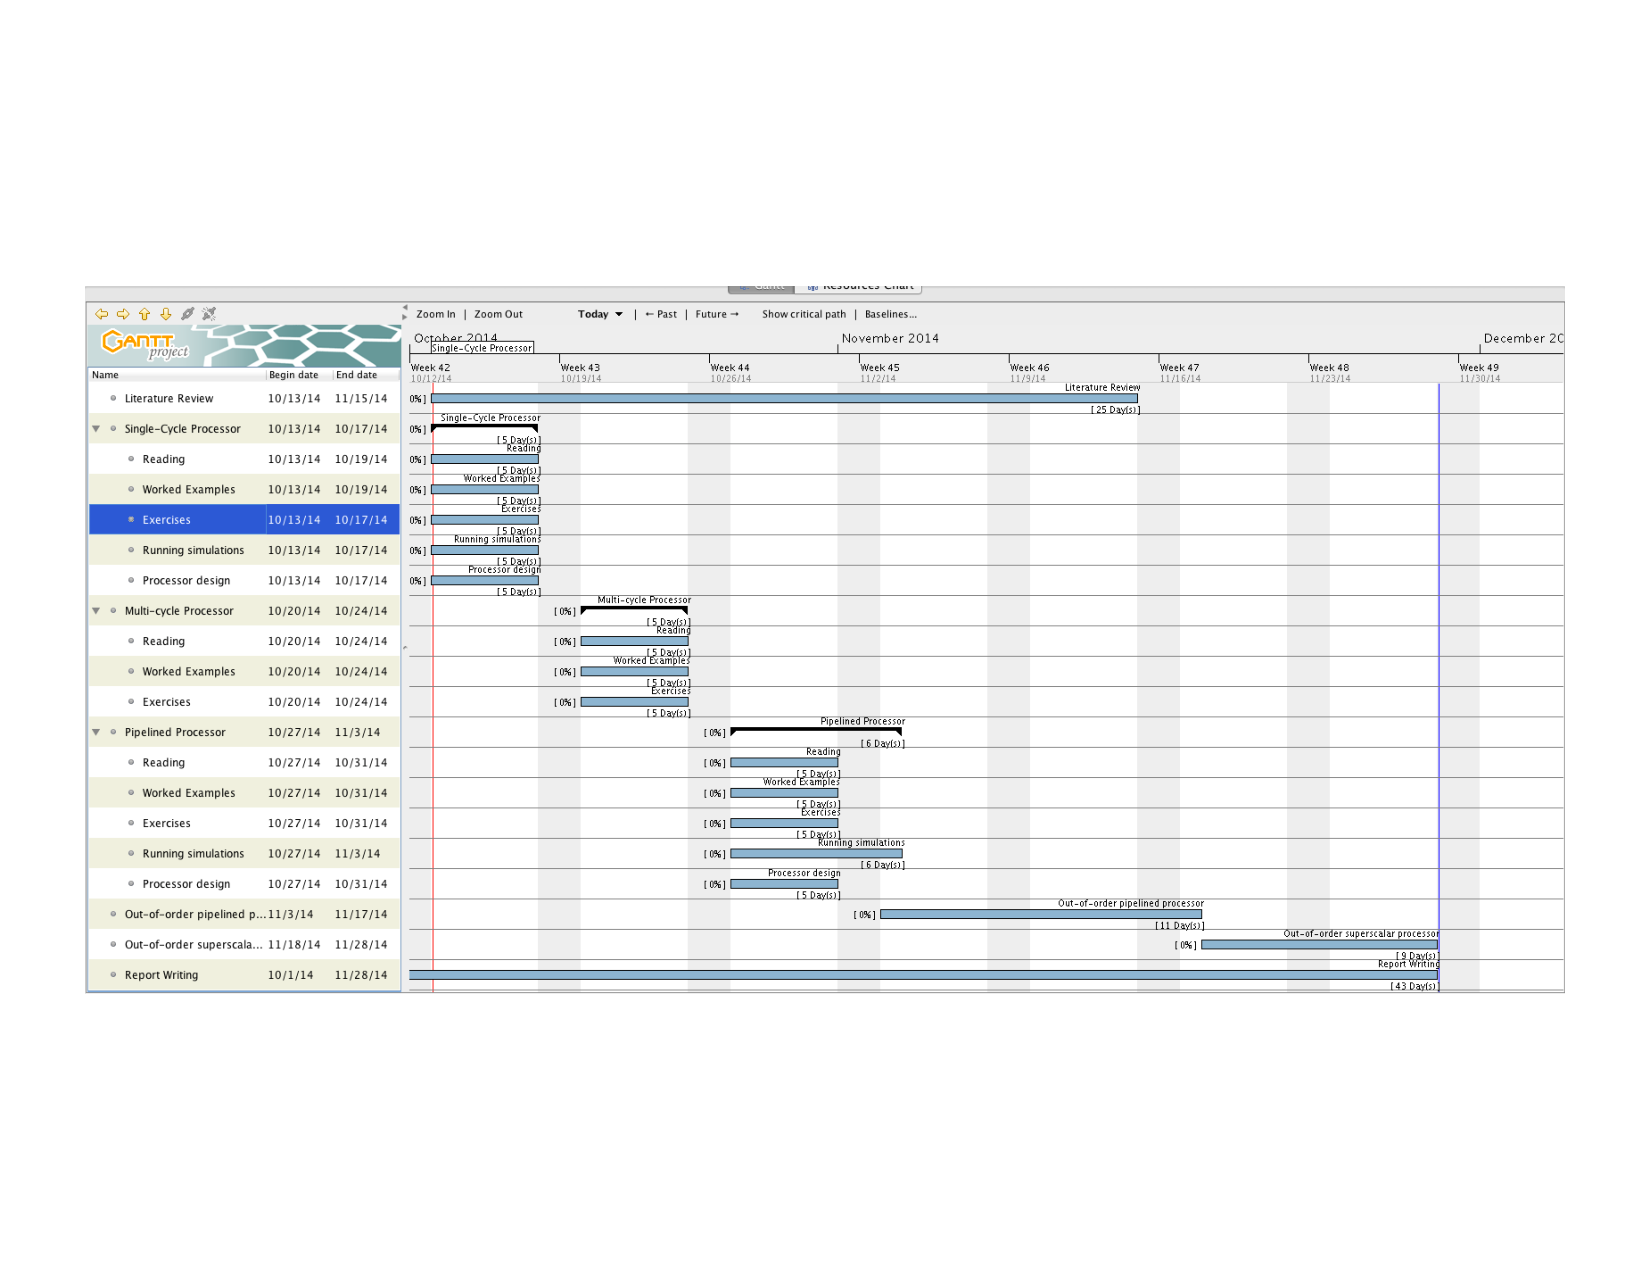
\includegraphics[width=6in]{./pics/gantt-chart}
\caption{This Gantt chart shows the project schedule.}
\label{fig:ganttchart}
\end{figure}

%%%%%%%%%%%%%%%%%%%%%%%%%%%%%%%%%%%%%%%%%%%
%\subsection{Roles and Personal Qualifications}
%\label{ssec:RolesandPersonalQualifications}



%%%%%%%%%%%%%%%%%%%%%%%%%%%%%%%%%%%%%%%%%%%
\subsection{Risk Management}
\label{ssec:RiskManagement}

A major risk to writing a good report for the class would include not being able to obtain experimental results from the processor design projects. If I cannot adequately test the designs by simulating them, I cannot verify if my processor designs are correct. In addition, I need to be able to find good samples of simple computer programs to test my processor design(s), so that I can use them as examples to explain the intricacies of modern processors. I would mitigate this risk by using very small snippets of computer programs that are used in my computer architecture classes to test my processors and demonstrate certain concepts. In addition, a minor risk to the project would be lost of data and text that I have written till date. I am addressing this risk by using an online repository (i.e., {\it Bitbucket}), based on cloud computing, to store various versions and modifications of my report and relevant class material (e.g., project proposal).




%%%%%%%%%%%%%%%%%%%%%%%%%%%%%%%%%%%%%%%%%%%
\section{Summary and Recommendation}
\label{sec:SummaryRecommendation}

This proposal summaries what report I would write, why is this report important, what I plan to do for my report writing process, and project management issues for writing this report. \\
\ \\
I strongly recommend that Prof. Richard McGuire approve this report proposal.







%	End left-alignment
\end{flushleft}


%%%%%%%%%%%%%%%%%%%%%%%%%%%%%%%%%%%%%%%%%%%%%
%%%%%%%%%%%%%%%%%%%%%%%%%%%%%%%%%%%%%%%%%%%%%
%
%	End of document
%
%	Inserting references
%
%%%%%%%%%%%%%%%%%%%%%%%%%%%%%%%%%%%%%%%%%%%%%
%%%%%%%%%%%%%%%%%%%%%%%%%%%%%%%%%%%%%%%%%%%%%
%	Beginning of BACK MATTER: bibliography, indexes and colophon
%\backmatter

%%%%%%%%%%%%%%%%%%%%%%%%%%%%%%%%%%%%%%%%%%%%%
{\linespread{1}
\bibliographystyle{plain}
\bibliography{/data/research/antipastobibtex/references}
}
%%%%%%%%%%%%%%%%%%%%%%%%%%%%%%%%%%%%%%%%%%%%%
\end{document}